\chapter{Produktivbetrieb}
    Das aus Kapitel \ref{Ergebnis} resultierende neuronale Netz sowie die Ergebnisauswertung dessen kann bisher nur begrenzt genutzt werden.
    Um diese Funktionen produktiv einsetzten zu können wird eine Schnittstelle zur einfachen Verwendung benötigt.
    
    An diese Schnittstelle werden folgende weitere Vorraussetzungen gestellt:
    \begin{description}
        \item[Echzeitanalyse] Es soll möglich sein Daten, beziehungsweise Batches in Echtzeit zu analysieren.
        \item[Periodenanalyse] Es soll möglich sein für beliebige historische Zeiträume Geräte zu klassifizieren.
        \item[Performance] Es sollte möglich sein lange Zeitreihen mit sehr vielen Daten auch noch in annehmbarer Zeit auszuwerten. Zudem sollte es möglich sein Zeitreihen in Echtzeit zu analysieren.
        \item[Tests] Um Fehler zu verhindern und ein stabiles und sicheres Programm zu entwickeln sollen wichtige fehleranfällige Funktionalitäten getestet werden.
    \end{description}
    
    \subsection{Implementierung}

        \begin{figure}[h]
            \centering
            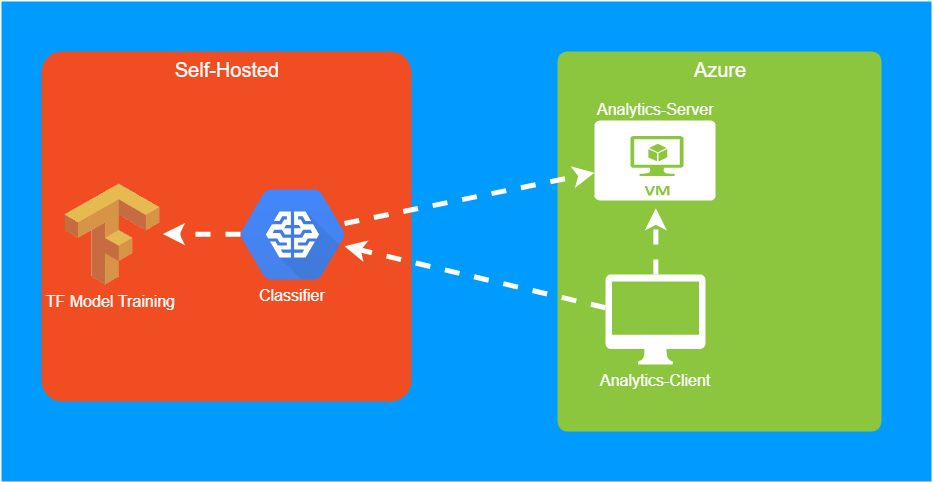
\includegraphics[width=1.0\textwidth]{ArchitectureProduct}
            \caption{Architektur zum Produktivbetrieb \protect\cite{DrawIO}, \protect\cite{Tensorflow}}
            \label{fig:ArchitectureTraining}
        \end{figure}

        Aufgrund besserer Performance und Einheitlichkeit mit der Daten-API wird eine Socekt.IO-API anstatt einer gebräuchlicheren REST-API gewählt.
        Die Spezifikation dieser Schnittstelle wird, wie in Abschnitt \ref{API-Spezifikation} beschrieben, festgelegt. 
        Somit ist die Echtzeitanalyse sowie die Periodenanalyse mit möglichst wenig Mehraufwand abgebildet.
        \newline

        Durch das Verwenden von Tensorflow und dessen Unterstützungseinschränkungen\footnote{https://www.tensorflow.org/install/} steht eine begrenzte Anzhal an Ansätzen zur Wahl.
        Es ist möglich die Architektur auf Python, C oder GoLang aufzubauen.
        Da die Architektur die vorher beschriebenen Anforderungen erfüllen muss und eine einfache Benutzung der neuronalen Netze erlauben sollte, werden mögliche Architekturen auf diese Anforderungen geprüft.
        \newline

        Da der komplette Trainingsprozess bereits in Python implementiert wurde, werden erste Implementierungen dort getestet \footnote{https://github.com/schrodit/wesense-ml/tree/master/prod}.
        Jedoch ist Python schlecht geeignet für viele Anfragen mit großem Rechenaufwand, wie für die Vorbereitung der Daten erforderlich ist.
        Auch konnte das Auslagern der aufwendigen Rechenoperationen keine bessereren Ergebnissen liefern.
        Somit wird entschieden den Produktivbetrieb in GoLang zu implementieren.
        \newline

        Der Einsatz von GoLang kann alle benötigten Anforderungen erfüllen, auch wenn die Einbindung sowie der Support von Tensorflow nicht so gut ausfällt, wie es bei Python der Fall ist.
        Jedoch kann mit GoLang die essentielle Performanceanforderung ohne Probleme erfüllt werden und auch die Stabilität sowie die Fehleranfälligkeit wird dadurch erheblich verbessert.
        Die Implementierung (siehe \footnote{https://github.com/schrodit/wesense-ml/tree/master/go}) besteht aus drei essentiellen Bausteinen, welche in Module (Packages) aufgeteilt sind.
        Diese drei Grundbausteine bestehen aus der Datentransformation, der Klassifikation sowie dem Socket.IO-Server.
        \newline

        Da im Datentransformations-Modul die essentiellen und fehleranfälligen Funktionalitäten implementiert sind, sind Tests für dieses Modul besonders wichtig.
        Hier wird eine Testabdeckung von mehr als 70\% erreicht um die Funktionsfähigkeit sicherzustellen.
        \newline

        Um eine stabile, zuverlässige und fehlerfreie Applikation zu schaffen wird eine \ac{CI}-Umgebung eingeführt.
        Diese \ac{CI}-Umgebung führt bei jedem Commit alle Tests aus, kompiliert das Program und baut einen Docker-Container (siehe \footnote{https://github.com/schrodit/wesense-ml/blob/master/.drone.yml}) in einer isolierten, gleichartigen Umgebung.
        Somit kann eine gleichbleibend gute Qualität der Applikation sichergestellt werden.
    
    \subsection{Deployment}
        Die Bereitstellung der API wird als Docker-Container realisiert.
        Diese Deployment-Strategie bietet viele Vorteile wie Abstraktion von anderen Programmen eines Systems bei wenig Performance-Verlust, welcher bei der Echtzeitanalyse von Nöten ist.
        Außerdem ermöglicht es ein automatisches Deployment mit automatischer Lastverteilung in weitere Docker-Umgebungen.
        Somit wird zur Bereitstellung der API nur eine Dockerumgebung benötigt und kann sehr einfach auf weitere Server portiert werden.
                

    \subsection{API-Spezifikation}\label{API-Spezifikation}
        \subsubsection{Single Batch}
        \paragraph{Input:}

            \begin{lstlisting}[language=json,firstnumber=1]
Topic: "single-batch"
{
    "data": [
        {
            "u": float,
            "f": float,
            "h3": float,
            "h5": float,
            "h7": float,
            "h9": float,
            "h11": float,
            "h13": float,
            "h15": float,
        },
        .. x Batchsize
    ]
}
            \end{lstlisting}
        
            \paragraph{Output:}
        
            \begin{lstlisting}[language=json,firstnumber=1]
Topic: 'single-prediction'
{
    "data": float //- Prediction of Senseo
}
            \end{lstlisting}
    
        \subsubsection{Period}
            \paragraph{Input:}
    
                \begin{lstlisting}[language=json,firstnumber=1]
Topic: "period"
{
    "data": {
        "start": "DateTime2",
        "end": "DateTime2"
    }
}
                \end{lstlisting}
            
                \paragraph{Output:}
            
                \begin{lstlisting}[language=json,firstnumber=1]
Topic: 'period-prediction'
* Series of Predictions where 0: Senseo, 1: Microwave, 2: Bosch, 3: Undefined, for every second
{
    "data": [
        Int,
        ... end - start
        Int
    ]
}
                \end{lstlisting}
